\documentclass[a4paper,12pt]{article}
\usepackage[utf8]{vietnam}
\usepackage{hyperref}
\usepackage{graphicx}
\usepackage{xcolor}
\usepackage{subfigure}
\usepackage{float}
\usepackage{placeins}
\usepackage{caption}
\usepackage{tabularx}
\usepackage{algpseudocode}
\usepackage{algorithm}
\usepackage{gensymb}
\floatname{algorithm}{Procedure}
\newenvironment{varalgorithm}[1]
  {\algorithm\renewcommand{\thealgorithm}{#1}}
  {\endalgorithm}
\renewcommand{\algorithmicrequire}{\textbf{Input:}}
\renewcommand{\algorithmicensure}{\textbf{Output:}}
\hypersetup{
	pdfborder = {0 0 0}
}
\title{\textbf{Báo cáo Project cuối kì \\ Thực hành kiến trúc máy tính}}
\author{Họ tên: Phan Minh Anh Tuấn \\ MSSV: 20205227}
\date{}
\begin{document}
	\maketitle
	\noindent
    \textbf{Học phần} Thực hành kiến trúc máy tính - IT3280 \textbf{- Mã lớp} 131003\\
    \textbf{Nhóm 1:}
    \begin{enumerate}
        \item Phan Minh Anh Tuấn (20205227)
        \item Nguyễn Thị Hoài Linh (20205231)
    \end{enumerate}
    \newpage
	\tableofcontents
	\newpage
	\section{Curiosity Marsbot}
	\subsection{Đề bài}
	Xe tự hành Curiosity Marsbot chạy trên sao Hỏa, được vận hành từ xa bởi các lập trình viên trên Trái Đất. Bằng cách gửi đi các mã điều khiển từ một bàn phím ma trận, lập trình viên điều khiển quá trình di chuyển của Marbot như sau:
	\begin{table}[!h]
		% \centering
		\label{ba1}
		\begin{tabularx}{\textwidth}{|l|X|} \hline
			\textbf{Mã điều khiển} & \textbf{Ý nghĩa}  \\ \hline 
			1b4  & Marbot bắt đầu chuyển động \\ \hline
			c68 & Marbot đứng im\\  \hline
			444 & Rẽ trái 90$^{\circ}$ so với phương chuyển động gần đây và giữ hướng mới\\ \hline
			666 & Rẽ phải 90$^{\circ}$ so với phương chuyển động gần đây và giữ hướng mới\\ \hline
			dad & Bắt đầu để lại vết trên đường\\  \hline
			cbc & Chấm dứt để lại vết trên đường\\  \hline
			999 & 
			Tự động quay trở lại theo lộ trình ngược lại. Không vẽ vết, không nhận mã khác cho tới khi kết thúc lộ trình ngược. 
			
			Mô tả: Marsbot được lập trình để nhớ lại toàn bộ lịch sử các mã điều khiển và khoảng thời gian giữa các lần đổi mã. Vì vậy, nó có thể đảo ngược lại lộ trình để quay về điểm xuất phát (dù có thể lệch một chút do hàm syscall sleep không thực sự thời gian thực)
			\\ \hline 
		\end{tabularx}
	\end{table}
	\noindent
	\\
	Sau khi nhận mã điều khiển, Curiosity Marsbot sẽ không xử lý ngay, mà phải đợi lệnh kích hoạt mã từ bàn phím Keyboard \& Display MMIO Simulator. Có 2 lệnh như vậy bao gồm:
	\begin{table}[!h]
		% \centering
		\label{ba1}
		\begin{tabularx}{\textwidth}{|l|X|} \hline
			\textbf{Kích hoạt mã} & \textbf{Ý nghĩa}  \\ \hline 
			Phím Enter  & Kết thúc nhập mã và yêu cầu Marbot thực thi \\ \hline
			Phím Del & Xóa toàn bộ mã điều khiển đang nhập dở dang\\  \hline
		\end{tabularx}
	\end{table}
	\\
	\noindent
	Hãy lập trình để Marsbot có thể hoạt động như đã mô tả. \\
	Đồng thời bổ sung thêm tính năng: mỗi khi gửi một mã điều khiển cho Marsbot, hiển thị mã đó lên màn hình console để người xem có thể giám sát lộ trình của xe.
	\clearpage
	\subsection{Ý tưởng}
	    Chương trình vận hành Curiosity Marsbot sẽ thực hiện ngắt (interrupt) mỗi khi nhận tín hiệu từ bên ngoài (khi có bất kỳ phím nào được bấm trên bàn phím ma trận), kiểm tra và lấy vào từng ký tự trong mã điều khiển hoặc đọc vào lệnh kích hoạt mã. \\ \\
	    Để biết cần điều khiển Marsbot ra sao, ta sẽ xây dựng chương trình con so sánh mã vừa nhập với các mã điều khiển quy định sẵn. Sau đó, từ chương trình chính ta sẽ nhảy đến các chương trình con thực hiện chức năng tương ứng (thực thi mã điều khiển, lưu trữ lịch sử điều khiển, xóa mã điều khiển).\\ \\
	    Để Marsbot có thể quay trở lại theo lộ trình ngược với ban đầu,  đường đi của Marsbot sẽ được lưu vào một mảng bằng cách: sau mỗi điều khiển rẽ trái/phải, ta sẽ lưu lại tọa độ (x,y) của điểm đầu tiên sau khi rẽ và hướng của Marbots khi đó. Nhờ vậy, ta có thể điều khiển Marsbot đi ngược lại bằng cách quay 180 độ và chuyển động đến khi về tọa độ cũ.\\ \\
	    \noindent
	    Chương trình sử dụng các công cụ sau:
	    \begin{itemize}
	    \item Marsbot: Giả lập robot
	    \item Digital Lab Sim: Nhập mã điều khiển
	    \item Keyboard and Display MMIO Simuator: Nhập lệnh kích hoạt
	    \item Console: Hiển thị mã điều khiển
	    \end{itemize}
	\clearpage
	\subsection{Khai báo và khởi tạo biến}
	    \FloatBarrier
        \begin{figure}[ht!]
    	    \centerline{\fbox{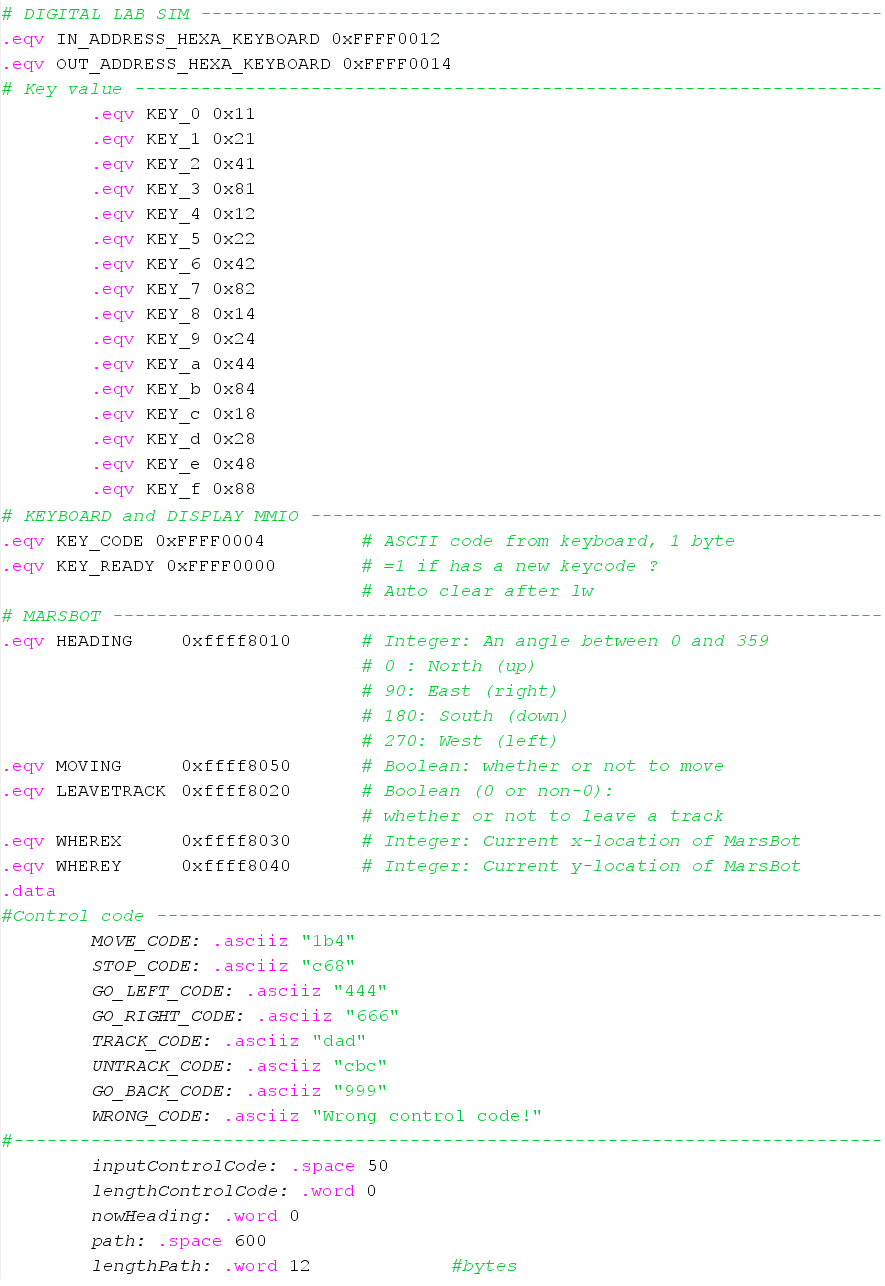
\includegraphics[width=0.92\textwidth]{bai1/01-khai-bao.png}}}
    	    \caption{Khai báo các địa chỉ, mã điều khiển và biến dùng trong chương trình}
    	    \label{fig:bai100}
        \end{figure}
        \noindent
	    Chương trình sử dụng các biến:
	    \begin{itemize}
	        \item inputControlCode: Mã điều khiển người dùng nhập vào
	        \item lengthControlCode: Độ dài mã điều khiển người dùng nhập vào	   
	        \item nowHeading: Hướng của Marsbot
	        \item path: Đường đi của Marsbot
	        \item lengthPath: Độ dài đường đi của Marsbot
	    \end{itemize}
	    Chi tiết về biến path và lengthPath: \\
	    Đường đi của Marsbot là một đường gấp khúc và được lưu vào mảng path theo từng khúc của đường đi. Mỗi khúc là một đoạn thẳng - đoạn đường giữa hai lần rẽ của Marsbot. Mỗi khúc được lưu dưới dạng 1 structure như sau: \{x, y, z\}, trong đó: 	
	    \begin{itemize}
	        \item x, y là tọa độ điểm đầu tiên của khúc
	        \item z là hướng của khúc đó
	    \end{itemize}
	    Lưu mỗi thành phần cần 1 word = 4 bytes nên lưu 1 structure cần 3 (words) x 4 (bytes) = 12 bytes. Mặc định structure đầu tiên là \{0,0,0\} và độ dài đường đi ngay khi bắt đầu là 12 bytes.
	\subsection{Cách thức thực hiện}
	    \begin{itemize}
	    	\item \textbf{Bước 1:} Chương trình cho phép mỗi khi người dùng nhập 1 kí tự từ \textit{Digital Lab Sim} thì sẽ tạo ra ngắt để lưu kí tự được nhập vào bộ nhớ, tạo nên đoạn mã điều khiển.
	    	\item \textbf{Bước 2:} Kiểm tra liên tục kí tự nhập vào ở \textit{Keyboard and Display MMIO Simulator}. Nếu phím Delete được nhấn, thực hiện xóa toàn bộ mã điều khiển đang nhập. Nếu phím Enter được nhấn, chuyển sang bước 3. Nếu không phải hai phím trên được nhấn, quay lại bước 1.
	    	\item \textbf{Bước 3:} Trước tiên kiểm tra độ dài mã điều khiển có đúng bằng 3 hay không, nếu không thì thông báo lỗi và chuyển sang bước 4. Sau đó, lần lượt kiểm tra mã điều khiển vừa nhập vào trùng với mã điều khiển nào đã quy định sẵn. Nếu không phát hiện mã vừa nhập trùng với bất kỳ mã điều khiển nào thì thông báo lỗi và chuyển sang bước 4. Nếu tìm được mã điều khiển trùng với mã người dùng nhập thì thực hiện điều khiển theo quy định.
    		\item \textbf{Bước 4:} In ra console mã điều khiển đã nhập và xóa lưu trữ trong bộ nhớ.
	    \end{itemize}
	    \FloatBarrier
        \begin{figure}[ht!]
    	    \centerline{\fbox{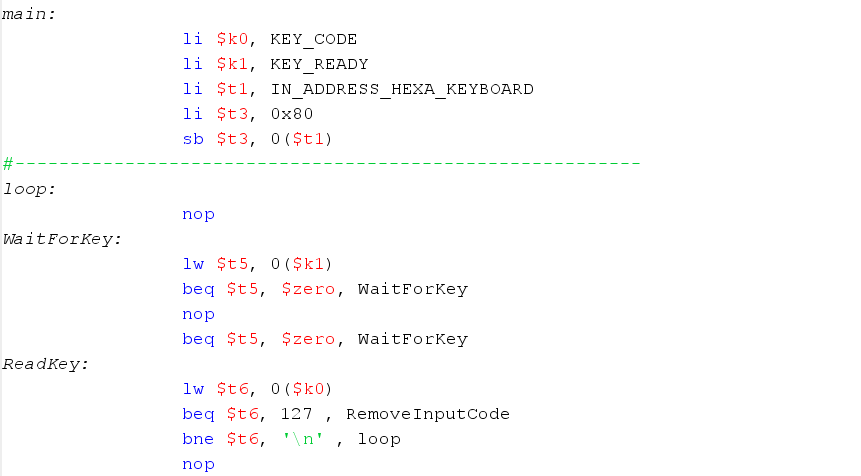
\includegraphics[width=0.92\textwidth]{bai1/02-main-1.png}}}
    	    \caption{Kiểm tra phím được nhấn ở Digital Lab Sim và Keyboard \& Display MMIO}
    	    \label{fig:bai100}
        \end{figure}
        \FloatBarrier
        \begin{figure}[ht!]
    	    \centerline{\fbox{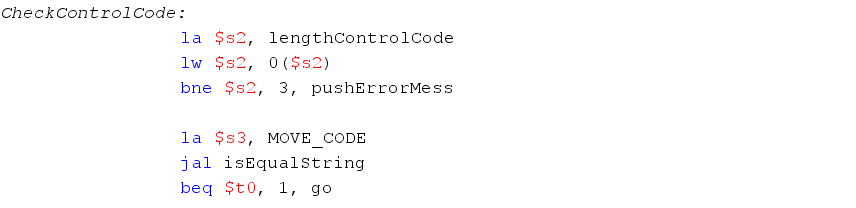
\includegraphics[width=0.92\textwidth]{bai1/03-main-2.png}}}
    	    \caption{Kiểm tra mã điều khiển (kiểm tra độ dài và minh họa 1 trường hợp so sánh với 1 mã điều khiển)}
    	    \label{fig:bai100}
        \end{figure}
        \FloatBarrier
        \begin{figure}[ht!]
    	    \centerline{\fbox{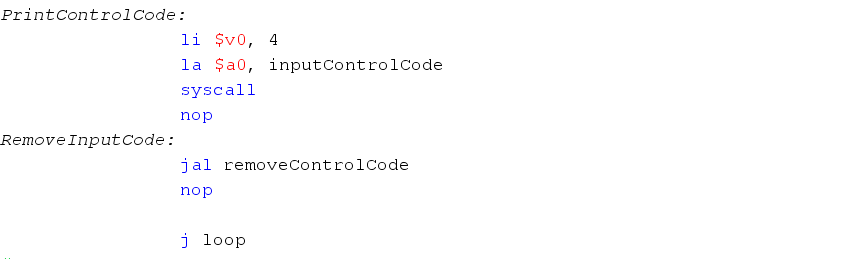
\includegraphics[width=0.92\textwidth]{bai1/04-main-3.png}}}
    	    \caption{In mã điều khiển ra console và xóa toàn bộ mã điều khiển nhập vào}
    	    \label{fig:bai100}
        \end{figure}
    	\clearpage
    	\noindent
    	\textbf{Trong đó:}
    	\begin{itemize}
    	    \item \$t5: KEY\_READY, bằng 1 khi có một phím được nhấn, tự động trở về 0 sau lệnh lw
    	    \item \$t6: KEY\_CODE, mã ASCII của phím được nhấn
    	    \item \$s2: Độ dài của mã người dùng nhập
    	    \item \$s3: Địa chỉ các mã điều khiển quy định sẵn
    	    \item \$t0: Biến đánh dấu mã người dùng nhập giống hay khác mã điều khiển đã quy định, bằng 1 khi hai mã giống nhau, ngược lại bằng 0
    	\end{itemize}
    	
    \clearpage
	\subsection{Các chương trình con}
	\subsubsection{isEqualString}
	    \textbf{Ý nghĩa:} So sánh mã điều khiển mà người dùng nhập vào với một mã điều khiển quy định sẵn.\\
	    \textbf{Đầu vào:} 
	    \begin{itemize}
            \item \$s1: Địa chỉ của mã mà người dùng nhập vào
            \item \$s3: Địa chỉ của mã điều khiển để so sánh với mã người dùng nhập
        \end{itemize}
        \textbf{Đầu ra:}
        \begin{itemize}
            \item \$t0: Nhận giá trị 1 nếu hai mã giống nhau, ngược lại nhận giá trị 0        
        \end{itemize}
        \FloatBarrier
        \begin{figure}[ht!]
    	    \centerline{\fbox{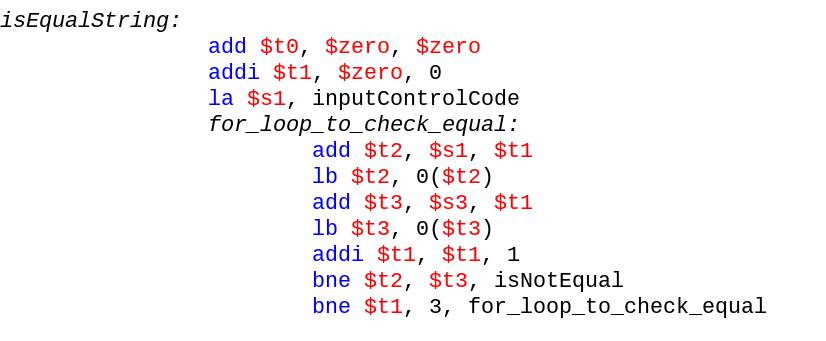
\includegraphics[width=0.8\textwidth]{bai1/05-isEqualString.png}
    	    }}
    	    \caption{Hàm isEqualString}
    	    \label{fig:bai100}
        \end{figure}
        \FloatBarrier
        \begin{figure}[ht!]
    	    \centerline{\fbox{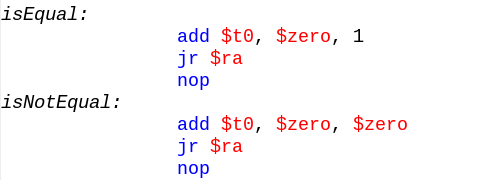
\includegraphics[width=0.8\textwidth]{bai1/06-isEqual.png}
    	    }}
    	    \caption{Hàm isEqual và isNotEqual}
    	    \label{fig:bai100}
        \end{figure}
        \noindent
	    \textbf{Giải thích:} Khởi tạo một biến i = 0, biến này sẽ tăng thêm 1 mỗi khi duyệt qua một ký tự. Lần lượt so sánh từng ký tự của mã nhập vào \textbf{inputControlCode} với mã điều khiển \textbf{s} bằng một vòng lặp. Nếu phát hiện hai ký tự khác nhau, lập tức nhảy đến hàm \textbf{isNotEqual} để gán \$t0 = 0. Nếu không phát hiện hai ký tự nào khác nhau cho đến khi biến i = 3, tức bằng độ dài mã, thì hai mã là giống nhau, ta nhảy đến hàm \textbf{isEqual} để gán \$t0 = 1. 
	\subsubsection{go, stop}
	    \textbf{Ý nghĩa:} Điều khiển Marsbot bắt đầu di chuyển (go) hoặc dừng lại (stop).\\
        \FloatBarrier
        \begin{figure}[ht!]
    	    \centerline{\fbox{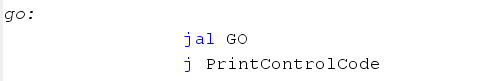
\includegraphics[width=0.92\textwidth]{bai1/08-go.png}
    	    }}
    	    \caption{Hàm go}
    	    \label{fig:bai100}
        \end{figure}
        \begin{figure}[ht!]
    	    \centerline{\fbox{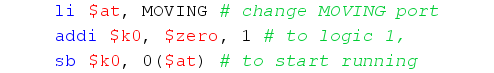
\includegraphics[width=0.92\textwidth]{bai1/09-GO.png}
    	    }}
    	    \caption{Hàm GO}
    	    \label{fig:bai100}
        \end{figure}
        \noindent
	    \textbf{Giải thích:} Load giá trị 1 vào địa chỉ MOVING (0xffff8050) khi muốn Marsbot di chuyển hoặc giá trị 0 khi muốn Marsbot dừng lại.
	    
	    \clearpage
    	\subsubsection{track, untrack}
	    \textbf{Ý nghĩa:} Điều khiển Marsbot bắt đầu (track) hoặc chấm dứt (untrack) để lại vết trên đường.\\
        \FloatBarrier
        \begin{figure}[ht!]
    	    \centerline{\fbox{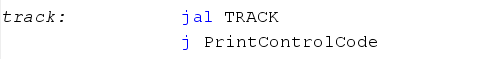
\includegraphics[width=0.92\textwidth]{bai1/10-track.png}
    	    }}
    	    \caption{Hàm track}
    	    \label{fig:bai100}
        \end{figure}
        \begin{figure}[ht!]
    	    \centerline{\fbox{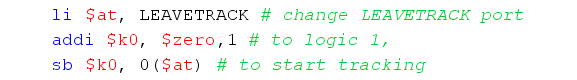
\includegraphics[width=0.92\textwidth]{bai1/11-TRACK.png}
    	    }}
    	    \caption{Hàm TRACK}
    	    \label{fig:bai100}
        \end{figure}
        \noindent
	    \textbf{Giải thích:} Load giá trị 1 vào địa chỉ LEAVETRACK (0xffff8020) khi muốn Marsbot để lại vết hoặc giá trị 0 khi muốn Marsbot dừng để lại vết.
	   \clearpage
	\subsubsection{goLeft, goRight}
	    \textbf{Ý nghĩa:} Điều khiển Marsbot rẽ trái (goLeft) hoặc rẽ phải (goRight).\\
	    \textbf{Đầu vào:} 
	    \begin{itemize}
            \item \$s6: nowHeading, hướng hiện tại của Marsbot
        \end{itemize}
        \FloatBarrier
        \begin{figure}[ht!]
    	    \centerline{\fbox{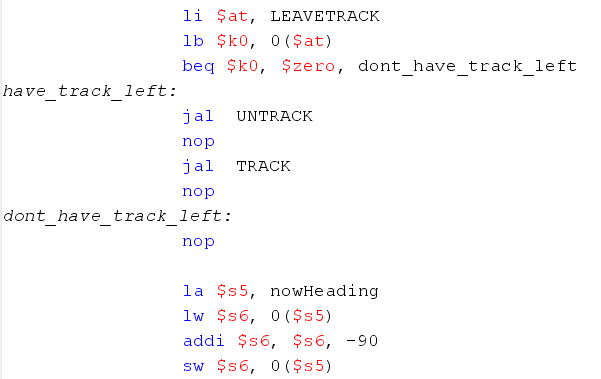
\includegraphics[width=0.8\textwidth]{bai1/12-goLeft.png}
    	    }}
    	    \caption{Hàm goLeft}
    	    \label{fig:bai100}
        \end{figure}
        \begin{figure}[ht!]
    	    \centerline{\fbox{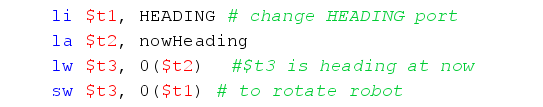
\includegraphics[width=0.8\textwidth]{bai1/13-ROTATE.png}
    	    }}
    	    \caption{Hàm ROTATE}
    	    \label{fig:bai100}
        \end{figure}
        \noindent
	    \textbf{Giải thích:} 
	    \begin{itemize}
	        \item Trước khi thực hiện quay trái/phải, ta cần kiểm tra hiện tại Marsbot có để lại vết khi di chuyển không. Nếu có thì phải thực hiện ngắt track cũ và vẽ lại track mới để không gặp hiện tượng track cũ bị thay đổi theo hướng di chuyển mới của Marsbot, sau đó mới thực hiện thay đổi hướng. Ngược lại, ta thay đổi hướng của Marsbot luôn.
	        \item Giảm biến nowHeading đi 90$^{\circ}$ để quay Marsbot sang trái hoặc tăng biến nowHeading thêm 90$^{\circ}$ để quay Marsbot sang phải.
	        \item Gọi hàm ROTATE để thực hiện xoay Marsbot. Hàm ROTATE sẽ load giá trị nowHeading vào địa chỉ HEADING (0xffff8010) để thay đổi hướng của Marsbot.
	        \item Mỗi khi thực hiện rẽ trái/phải, ta cần lưu lại hướng và vị trí của Marsbot để sau đó có thể điều khiển Marsbot quay trở lại theo lộ trình ngược lại, việc này được thực hiện nhờ chương trình con \textbf{storePath} sẽ được trình bày sau.
	    \end{itemize} 
	\clearpage
	\subsubsection{goBack}
	    \textbf{Ý nghĩa:} Điều khiển Marsbot quay trở lại theo lộ trình ngược lại.\\ \\
	    \textbf{Đầu vào:} 
	    \begin{itemize}
            \item \$s5: lengthpath, độ dài của biến path lưu đường đi của Marsbot
            \item \$s7: Biến path lưu đường đi của Marsbot
        \end{itemize}
	    \FloatBarrier
        \begin{figure}[ht!]
    	    \centerline{\fbox{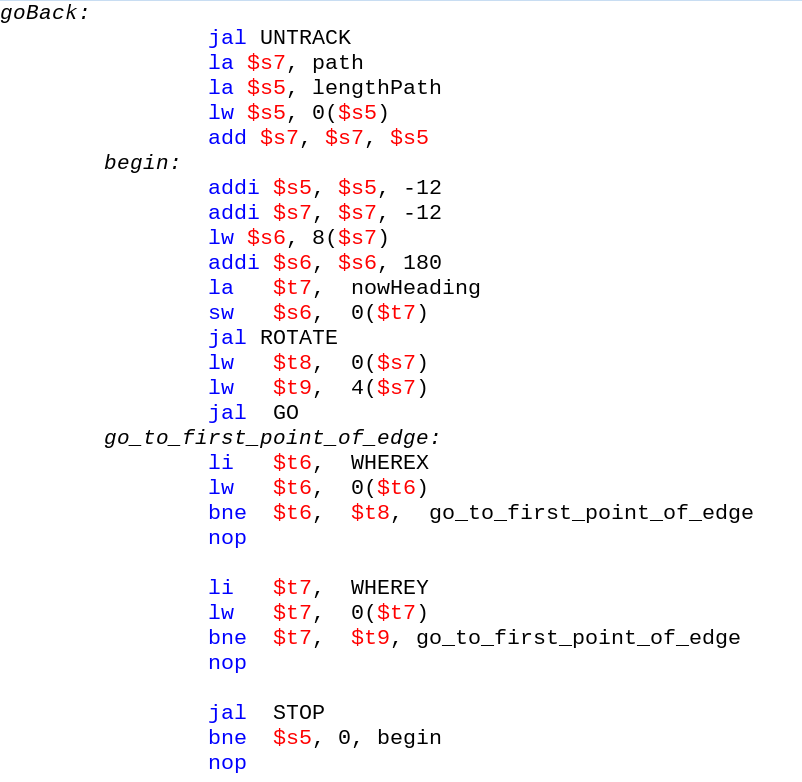
\includegraphics[width=0.9\textwidth]{bai1/14-goBack_1.png}
    	    }}
    	    \label{fig:bai100}
        \end{figure}
        \clearpage
        \begin{figure}[ht!]
    	    \centerline{\fbox{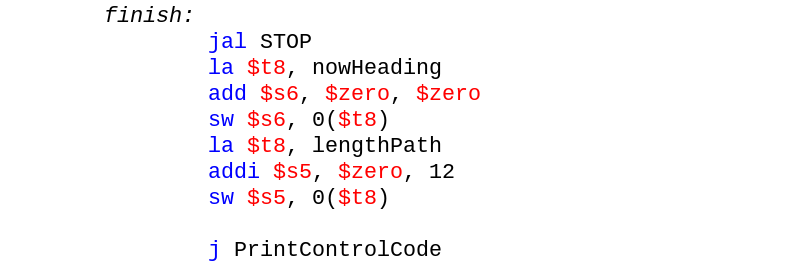
\includegraphics[width=0.85\textwidth]{bai1/14-goBack_3.png}
    	    }}
    	    \caption{Hàm goBack}
    	    \label{fig:bai100}
        \end{figure}
        \noindent
	    \textbf{Giải thích:}
	        \begin{itemize}
	            \item Bước 1: Ngừng để lại track.
	            \item Bước 2: Giảm độ dài đường đi lengthPath (\$s5) đi 12, đồng thời lùi về vị trí chứa thông tin lần rẽ cuối cùng.
	            \item Bước 3: Lấy thông tin về hướng của Marsbot ở lần rẽ cuối cùng từ \$s7, tăng hướng đó thêm 180$^{\circ}$ để quay MarsBot ngược lại.
	            \item Bước 4: Lấy thông tin về tọa độ x,y của điểm đầu tiên (lưu vào \$t8,\$t9) ở lần rẽ cuối cùng từ \$s7. Cho Marsbot di chuyển. Trong khi đó, liên tục lấy tọa độ x,y hiện tại (lưu vào \$t6,\$t7) của Marsbot và so sánh hai cặp tọa độ (\$t6 với \$t8, \$t7 với\$t9) đến khi chúng bằng nhau thì cho Mars dừng lại.
	            \item Bước 5: So sánh độ dài đường đi (\$s5) với 0. Khi \$s5 = 0 là đã quay ngược lại hết lộ trình, ta cập nhật lại hướng (= 0$^{\circ}$) cho Marsbot và độ dài đường đi cập nhật bằng 12 bytes. Ngược lại, ta lặp lại từ bước 2.
	        \end{itemize}
	\clearpage
	\subsubsection{storePath}
	    \textbf{Ý nghĩa:} Lưu các thông tin về đường đi của Marsbot.\\
	    \textbf{Đầu vào:} 
	    \begin{itemize}
            \item \$s1: Tọa độ x hiện tại của MarsBot
            \item \$s2: Tọa độ y hiện tại của MarsBot
            \item \$s4: Hướng hiện tại của Marsbot
            \item \$s3: lengthpath, độ dài của biến path lưu đường đi của Marsbot
            \item \$t4: Địa chỉ biến path lưu đường đi của Marsbot
        \end{itemize}
        \FloatBarrier
        \begin{figure}[ht!]
    	    \centerline{\fbox{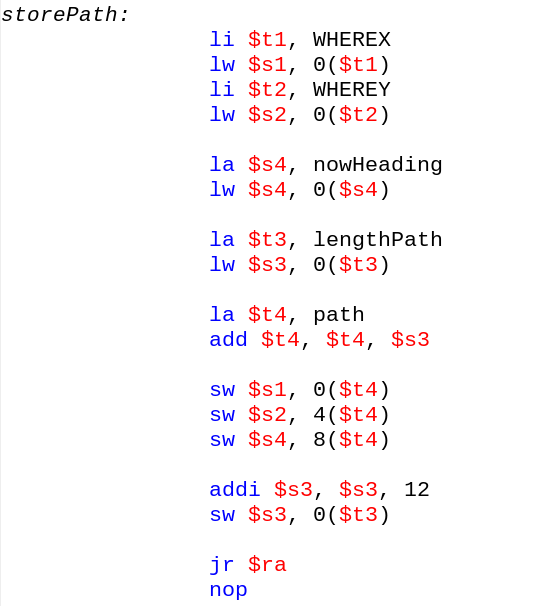
\includegraphics[width=0.8\textwidth]{bai1/15-storePath.png}
    	    }}
    	    \caption{Hàm storePath}
    	    \label{fig:bai100}
        \end{figure}
        \clearpage
        \noindent
	    \textbf{Giải thích:}
	        \begin{itemize}
	            \item Bước 1: Lấy thông tin về tọa độ x,y, hướng hiện tại của Marsbot từ địa chỉ WHEREX, WHEREY, nowHeading.
	            \item Bước 2: Lấy địa chỉ biến path cộng với giá trị độ dài đường đi hiện tại để đi đến cuối mảng path và bắt đầu lưu các thông tin: x, y, hướng. 
	            \item Bước 3: Cập nhật độ dài đường đi tăng thêm 12 bytes.
	        \end{itemize}	
	\subsubsection{pushErrorMess}
	    \textbf{Ý nghĩa:} Thông báo mã điều khiển vừa nhập vào không đúng.\\
        \FloatBarrier
        \begin{figure}[ht!]
    	    \centerline{\fbox{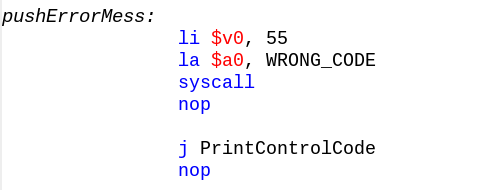
\includegraphics[width=0.92\textwidth]{bai1/16-pushErrorMess.png}}}
    	    \caption{Hàm pushErrorMess}
    	    \label{fig:bai100}
        \end{figure}
        \noindent
	    \textbf{Giải thích:} Sử dụng các hàm syscall 55 để in thông báo qua một hộp thoại và quay lại chương trình chính tại vị trí hàm PrintControlCode.
	\clearpage
	\subsubsection{removeControlCode}
	    \textbf{Ý nghĩa:} Xóa toàn bộ mã điều khiển đang nhập.\\
	    \textbf{Đầu vào:} 
	    \begin{itemize}
            \item \$t3: Độ dài mã điều khiển đang nhập
            \item \$s1: Địa chỉ lưu mã điều khiển đang nhập
        \end{itemize}
        \FloatBarrier
        \begin{figure}[ht!]
    	    \centerline{\fbox{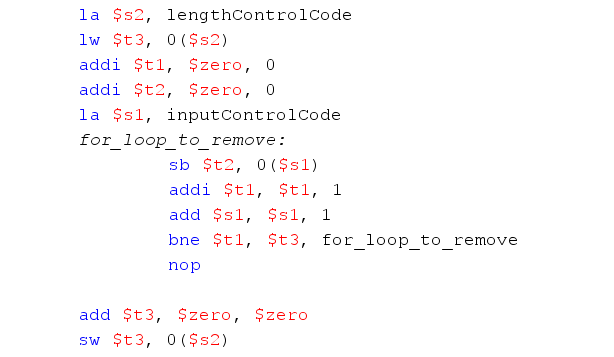
\includegraphics[width=0.92\textwidth]{bai1/17-removeControlCode.png}
    	    }}
    	    \caption{Hàm removeControlCode}
    	    \label{fig:bai100}
        \end{figure}
        \noindent
	    \textbf{Giải thích:} Khởi tạo một biến chạy i = 0 (\$t1 = 0). Dùng một vòng lặp để lần lượt gán các ký tự trong mã đang nhập bằng ‘\textbackslash0’ cho đến khi biến i > 3 thì dừng. Sau đó cập nhật lại độ dài mã điều khiển đang nhập về bằng 0.
	\clearpage
    \subsubsection{Chương trình con xử lý ngắt}
	    \textbf{Ý nghĩa:} Quét tìm phím được nhấn và chuyển từ mã của phím đó sang mã ký tự tương ứng lưu vào xâu mã điều khiển đang nhập.\\
	    Trong chương trình con xử lý ngắt, có 2 thao tác chính:
        \FloatBarrier
        \begin{figure}[ht!]
    	    \centerline{\fbox{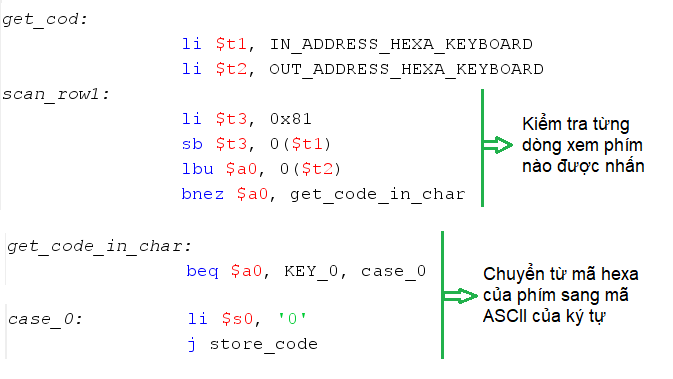
\includegraphics[width=0.8\textwidth]{bai1/18-get-cod.png}
    	    }}
    	    \caption{Hàm get\_cod}
    	    \label{fig:bai100}
        \end{figure}
        \FloatBarrier
        \begin{figure}[ht!]
    	    \centerline{\fbox{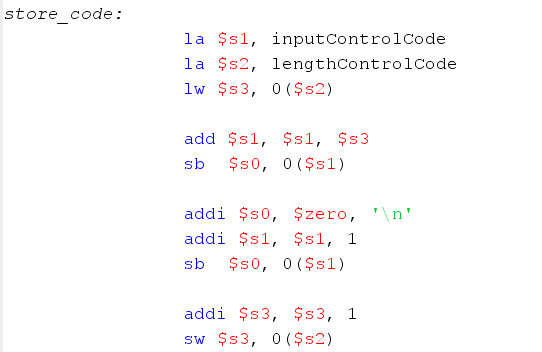
\includegraphics[width=0.8\textwidth]{bai1/19-store-code.png}
    	    }}
    	    \caption{Hàm store\_code}
    	    \label{fig:bai100}
        \end{figure}
        \clearpage
        \noindent
    {\textbf{a. get\_cod}} \\
                \textbf{Đầu ra:}
                \begin{itemize}
                    \item \$a0: Mã hexa của phím được nhấn
                    \item \$s0: Mã ASCII của ký tự tương ứng với phím được nhấn
                \end{itemize}
                \textbf{Giải thích:} Lần lượt quét các hàng của Digital Lab Sim để xem phím nào được nhấn: lưu mã của hàng vào địa chỉ IN\_ADDRESS\_HEXA\_KEYBOARD, sau đó load giá trị ở địa chỉ OUT\_ADDRESS\_HEXA\_KEYBOARD vào \$a0, nếu được giá trị khác 0 là đã có phím được nhấn, ta chuyển sang tìm mã ASCII của ký tự tương ứng với phím đó. So sánh \$a0 với mã hexa của các phím đã được khai báo ở đầu chương trình và gán cho \$s0 mã ASCII tương ứng.
                \\ \\
    \textbf{b. store\_code}\\
                \textbf{Đầu vào:}
                \begin{itemize}
                    \item \$s0: Mã ASCII của ký tự tương ứng với phím được nhấn
                    \item \$s1: Địa chỉ của mã điều khiển đang nhập (inputControlCode)
                    \item \$s3: Độ dài của mã điều khiển đang nhập
                \end{itemize}
                \textbf{Giải thích:} Lưu mã ASCII vừa tìm được trước đó vào cuối xâu inputControlCode và thêm ký tự '\textbackslash n' vào cuối xâu đó để khi in ra console thì các mã tách rời, dễ quan sát. Cuối cùng cập nhật độ dài của mã đang nhập tăng thêm 1.
    \clearpage
    \subsection{Kết quả}
    \FloatBarrier
        \begin{figure}[ht!]
    	    \centerline{\fbox{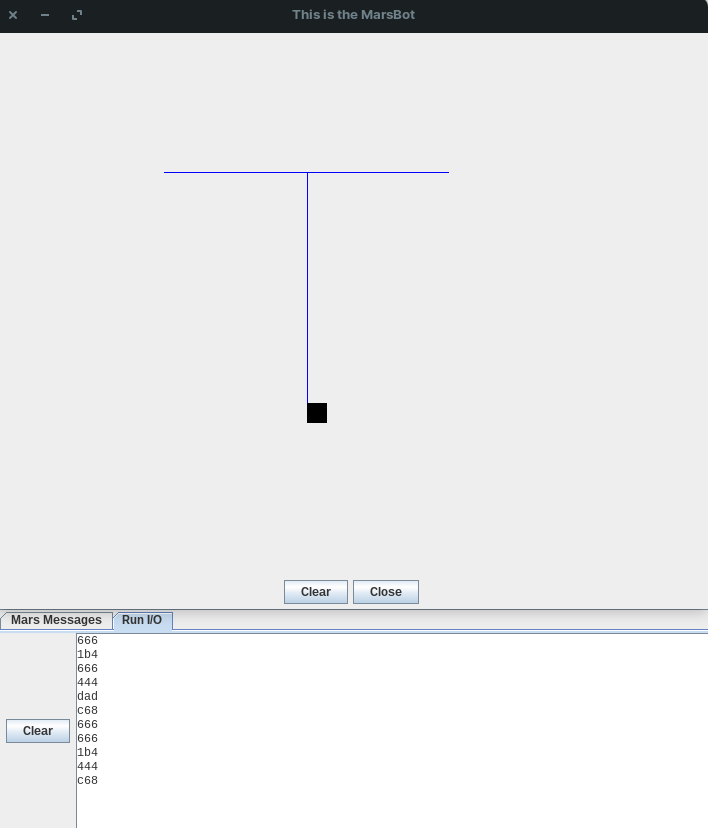
\includegraphics[width=0.9\textwidth]{bai1/Tuan.png}
    	    }}
    	    \caption{Kết quả bài 1}
    	    \label{fig:bai100}
        \end{figure}
        \noindent
    Điều khiển MarsBot di chuyển tạo thành hình chữ T trong tên "Phan Minh Anh Tuấn". 
	
	
	
	
	
	
	
	
	
	
	
	
	
	
	
	\clearpage
	\section{Vẽ hình trên màn hình Bitmap}
	\subsection{Đề bài}
	Viết một chương trình sử dụng MIPS để vẽ một quả bóng di chuyển trên màn hình mô phỏng Bitmap của Mars). Nếu đối tượng đập vào cạnh của màn hình thì sẽ di chuyển theo chiều ngược lại. \\
	Yêu cầu:
	\begin{itemize}
		\item Thiết lập màn hình ở kích thước 512x512. Kích thước 1 pixel 1x1.
		\item Quả bóng là một đường tròn
	\end{itemize}
	Chiều di chuyển phụ thuộc vào phím người dùng bấm, gồm có (di chuyển lên (w), di chuyển xuống (s), sang trái (a), sang phải (d) trong bộ giả lập Keyboard and Display MMIO Simulator). Tốc độ bóng di chuyển là không đổi. Vị trí bóng ban đầu ở giữa màn hình.
	\\ \\ \\ 
	\begin{figure}[!h]
    	\centerline{\fbox{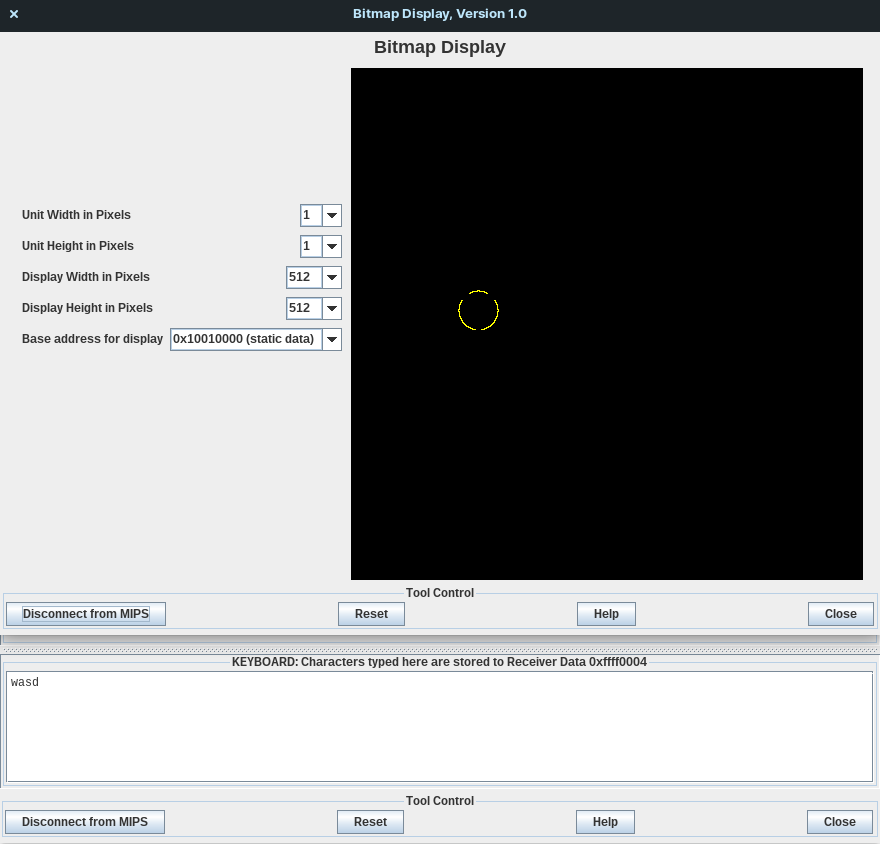
\includegraphics[width=0.73\textwidth]{bai2/bai2.png}}}
    	\caption{Giao diện chương trình bài 2}
    	\label{fig:bai6}
    \end{figure}
	\clearpage
	\subsection{Ý tưởng}
	Chương trình bao gồm hai công đoạn chính:
	\begin{itemize}
	    \item Vẽ hình tròn: Sử dụng \ref{alg:cap} với tâm là (256,256).
	    \item Điều khiển hình tròn: So sánh mã vừa nhập với các mã điều khiển quy định sẵn. Sau đó, từ chương trình chính sẽ nhảy đến các chương trình con thực hiện chức năng tương ứng (lên, xuống, sang trái, sang phải).
	\end{itemize}
	\begin{varalgorithm}{thuật toán Midpoint Circle}
	\caption{}
    \label{alg:cap}
    \begin{algorithmic}
    \Require $(x_0,y_0), r$
    \Ensure Hình tròn với tâm là $(x_0,y_0)$ bán kính r
    \State $x \gets r$
    \State $y \gets 0$
    \State $e \gets 0$
    \While{$x \geq y$}
    \State putpixel($x_0+x,y_0+y$)
    \State putpixel($x_0+y,y_0+x$)
    \State putpixel($x_0-y,y_0+x$)
    \State putpixel($x_0-x,y_0+y$)
    \State putpixel($x_0-x,y_0-y$)
    \State putpixel($x_0-y,y_0-x$)
    \State putpixel($x_0+y,y_0-x$)
    \State putpixel($x_0+x,y_0-y$)
    \If{$e \leq 0$}
        \State $y \gets y + 1$
        \State $e \gets e + 2y + 1$
    \Else
        \State $x \gets x - 1$
        \State $e \gets e - 2x - 1$
    \EndIf
    \EndWhile
    \end{algorithmic}
    \end{varalgorithm}
    Chương trình sử dụng các công cụ sau:
	\begin{itemize}
	    \item Bitmap Display: Hiển thị quả bóng
	    \item Keyboard and Display MMIO Simuator: Nhập mã điều khiển
	\end{itemize}
    \clearpage
    \subsection{Cách thức thực hiện}
    \begin{itemize}
        \item \textbf{Bước 1:} Vẽ hình tròn màu vàng với tâm là (256,256) và hiển thị lên Bitmap Display.
        \item \textbf{Bước 2:} Chương trình liên tục đọc phím mà người dùng nhập Keyboard and Display MMIO Simuator.
        \item \textbf{Bước 3:} So sánh phím được nhập với các mã điều khiển đã quy định. Nếu phím đó trùng với mã điều khiển a, d, w, s thì thực hiện di chuyển bóng tương ứng sang trái, sang phải, lên, xuống. Sau đó tiếp tục kiểm tra phím được nhập. 
    \end{itemize}
    
    
    \subsection{Các chương trình con}
    Triển khai \ref{alg:cap} để vẽ hình tròn thông qua ba hàm chính \textbf{DrawCircle},  \textbf{circleLoop} và \textbf{drawDot}
    \FloatBarrier
    \begin{figure}[ht!]
    	\centerline{\fbox{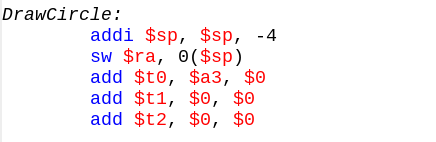
\includegraphics[width=0.7\textwidth]{bai2/drawcircle.png}}}
    	\caption{Khai báo các biến của chương trình vẽ hình tròn}
    	\label{fig:bai6}
    \end{figure}
    \noindent
    \textbf{Trong đó}:
    \begin{itemize}
        \item \$t0: Biến x, giá trị khởi tạo bằng r
        \item \$t1: Biến y, giá trị khởi tạo bằng 0
        \item \$t2: Biến e, giá trị khởi tạo bằng 0
    \end{itemize}
    \clearpage
    \subsubsection{circleLoop}
    \FloatBarrier
    \begin{figure}[ht!]
    	\centerline{\fbox{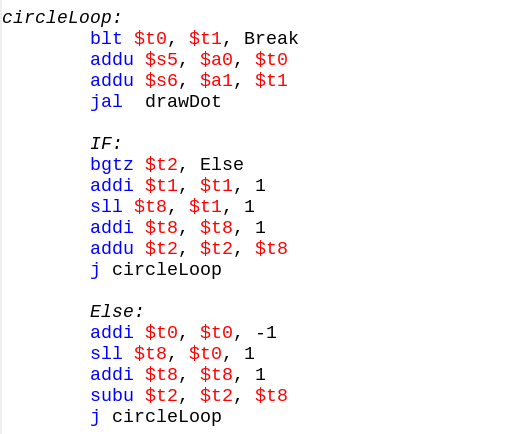
\includegraphics[width=0.7\textwidth]{bai2/circleloop.png}}}
    	\caption{Hàm circleLoop thực hiện vòng lặp khi $x \geq y$}
    	\label{fig:bai100}
    \end{figure}
    \noindent
    \textbf{Trong đó}:
    \begin{itemize}
        \item \$t0: Biến x, giá trị khởi tạo bằng r
        \item \$t1: Biến y, giá trị khởi tạo bằng 0
        \item \$t2: Biến e, giá trị khởi tạo bằng 0
        \item \$a0: Vị trí tọa độ tâm của x hiện tại 
        \item \$a1: Vị trí tọa độ tâm của y hiện tại
    \end{itemize}
    \textbf{Giải thích:}
    Hình \ref{fig:bai100} trình bày 1 trong số nhiều lần putpixel của  \ref{alg:cap} với:
    \begin{itemize}
        \item \$s5 = \$a0 + \$t1 = $x_0 + x$
        \item \$s6 = \$a1 + \$t0 = $y_0 + y$
    \end{itemize}
    Đoạn mã trên tương ứng với trường hợp putpixel($x_0+x,y_0+y$). \\ \\
    \textsf{Nếu} $e \leq 0$ (\$t2 $\leq$ 0) $\Rightarrow y = y + 1, e = e + 2y + 1$. \\ \\
    \textsf{Ngược lại} $\Rightarrow x = x - 1, e = e - 2x - 1$.  \\ \\
    Sau đó quay trở lại thực hiện vòng lặp cho đến khi điều kiện lặp $x \geq y$ không thỏa mãn.
    \subsubsection{Draw Dot}
    \FloatBarrier
    \begin{figure}[ht!]
    	\centerline{\fbox{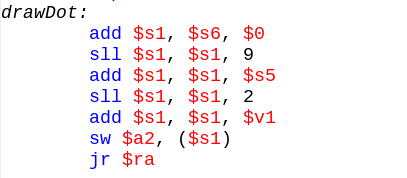
\includegraphics[width=0.7\textwidth]{bai2/drawdot.png}}}
    	\caption{Hàm drawDot}
    	\label{fig:bai7}
    \end{figure}
    \noindent
    \textbf{Trong đó}:
    \begin{itemize}
        \item \$v1: Địa chỉ của MONITOR$\_$SCREEN.
        \item \$a2: Giá trị màu vàng.
        \item \$s1: Địa chỉ pixel cần vẽ trên màn hình.
        \item \$s5: Toạ độ x cần vẽ được lấy từ hàm circleLoop tương ứng khi jal drawDot.
        \item \$s6: Toạ độ y cần vẽ được lấy từ hàm circleLoop tương ứng khi jal drawDot.
    \end{itemize}
    \textbf{Giải thích:} Do màn hình có kích thước 512x512 \\ \\
    $\Rightarrow$ Index 1 điểm trên màn hình $= y*512 + x$. \\
    $\Rightarrow$ Offset 1 điểm trên màn hình $= (y*512 + x) * 4$. \\ \\
    Sau đó lưu thông tin màu vàng vào \$s1 để vẽ lên Bitmap Display.
    \clearpage
    \subsubsection{Input}
    \FloatBarrier
    \begin{figure}[ht!]
    	\centerline{\fbox{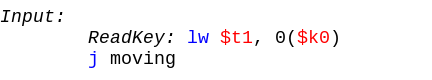
\includegraphics[width=0.7\textwidth]{bai2/input.png}}}
    	\caption{Hàm Input}
    	\label{fig:bai6}
    \end{figure}
    \noindent
    \textbf{Trong đó:}
    \begin{itemize}
        \item \$k0: Địa chỉ của KEY\_CODE, tại địa chỉ này chứa mã ASCII của ký tự người dùng nhập vào
    \end{itemize}
    \textbf{Giải thích:} Thực hiện đọc kí tự từ bàn phím qua thanh ghi \$k0, sau đó lưu vào thanh ghi \$t1.
    \subsubsection{Pause}
    \FloatBarrier
    \begin{figure}[ht!]
    	\centerline{\fbox{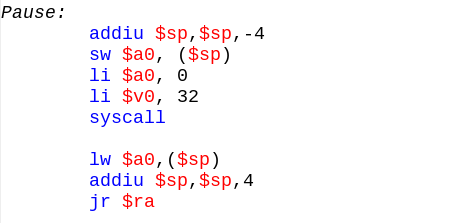
\includegraphics[width=0.7\textwidth]{bai2/pause.png}}}
    	\caption{Hàm Pause}
    	\label{fig:bai6}
    \end{figure}
    \noindent
    \textbf{Giải thích:} Điều chỉnh tốc độ di chuyển của quả bóng thông qua hàm sleep (syscall 32), tùy chỉnh thời gian thông qua \$a0.
    \clearpage
    \subsubsection{Moving}
    Kiểm tra phím nhập vào từ Keyboard \& Display MMIO Simulator để thực hiện 1 trong 4 chương trình con: \textbf{Left}, \textbf{Right}, \textbf{Down}, \textbf{Up}. \\
    Dưới đây sẽ trình bày về hàm \textbf{Left}, các hàm còn lại tương tự. \\
    \FloatBarrier
    \begin{figure}[ht!]
    	\centerline{\fbox{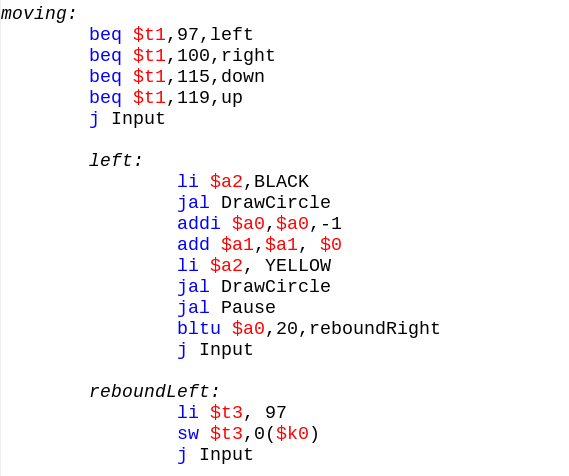
\includegraphics[width=0.7\textwidth]{bai2/moving.png}}}
    	\caption{Hàm moving}
    	\label{fig:bai6}
    \end{figure}
    \noindent
    \textbf{Trong đó:}
    \begin{itemize}
        \item \$a0: Tọa độ x của tâm hình tròn hiện tại
        \item \$a1: Tọa độ y của tâm hình tròn hiện tại
    \end{itemize}
    \textbf{Giải thích:}
    \begin{enumerate}
        \item Chuyển màu sắc của hình tròn (lưu trong thanh ghi \$a2) về màu đen cùng màu với nền, sau đó vẽ lại hình tròn. Bước này tương đương với việc xóa hình tròn trên màn hình.
        \item Dịch vị trí của tâm sang trái 1 đơn vị ($x_0 = x_0 - 1$).
        \item Chuyển lại màu sắc hình tròn về màu vàng. Sau đó vẽ lại hình tròn.
        \item Khi bóng đập vào tường, lúc này $x_0 < 20$. Thực hiện hàm reboundRight để di chuyển theo chiều ngược lại. 
    \end{enumerate}
\end{document}